\documentclass[10pt,twocolumn]{article}
\usepackage[margin=0.62in]{geometry}
\usepackage{graphicx}
\usepackage{booktabs}
\usepackage{enumitem}
\usepackage{titlesec}
\usepackage{xcolor}
\usepackage{caption}

\setlength{\columnsep}{0.22in}
\setlength{\parindent}{0pt}
\setlength{\parskip}{3pt}
\setlist[itemize]{leftmargin=*,nosep}
\titlespacing*{\section}{0pt}{6pt}{3pt}
\titlespacing*{\subsection}{0pt}{4pt}{2pt}
\captionsetup{font=scriptsize,labelfont=bf}

\begin{document}

\title{\vspace{-1.0cm}\textbf{Reddit Recommendation Analytics Dashboard Report}}
\author{Harsh Kaushik (2023AIB1006) \and Yash Hatwar (2023AIB1257) \and Arun (2023AIB1014)}
\date{}
\maketitle
\vspace{-0.65cm}

\section{Methodology}
The final aim of this project is to recommend what can be posted on Reddit by analyzing multiple signals: word popularity, engagement, sentiment, controversiality, and topic saturation. The system combines a batch/stream data pipeline, a FastAPI analytics layer, and a React dashboard. Reddit post and comment JSON data are loaded into a local SQLite warehouse using \texttt{backend/load\_historic.py}; live-style ingestion is supported by \texttt{backend/spark\_reddit\_metrics.py}, which uses Spark Structured Streaming and writes micro-batch aggregates into \texttt{reddit\_post\_facts} and \texttt{reddit\_comment\_facts}. The backend exposes filtered APIs for overview metrics, comment analytics, advanced feature insights, recommendation, retrieval, and explanation.

The sentiment methodology uses a lightweight lexicon-based approach. In \texttt{backend/main.py}, each Reddit title is tokenized, positive and negative word hits are counted, and sentiment is computed as \((positive-negative)/tokens\). Scores above zero are treated as positive, scores below zero are treated as negative, and zero is treated as neutral. These scores drive sentiment KPIs, the sentiment timeline, topic heatmaps, word sentiment-engagement scatter plots, best-topic recommendations, and avoid-topic rankings. Engagement is computed from post score, upvotes, and comments, while controversy is estimated as comments divided by absolute score plus one.

The React frontend in \texttt{frontend/src/pages} renders four user workflows: Reddit dashboard, comment analysis, advanced features, and action recommender. Shared chart components include time-series area charts, donut charts, bar charts, heatmaps, and scatter plots. Filters for year and month are passed into backend query parameters, allowing the same visual components to update for different time windows.

\begin{figure}[h]
  \centering
  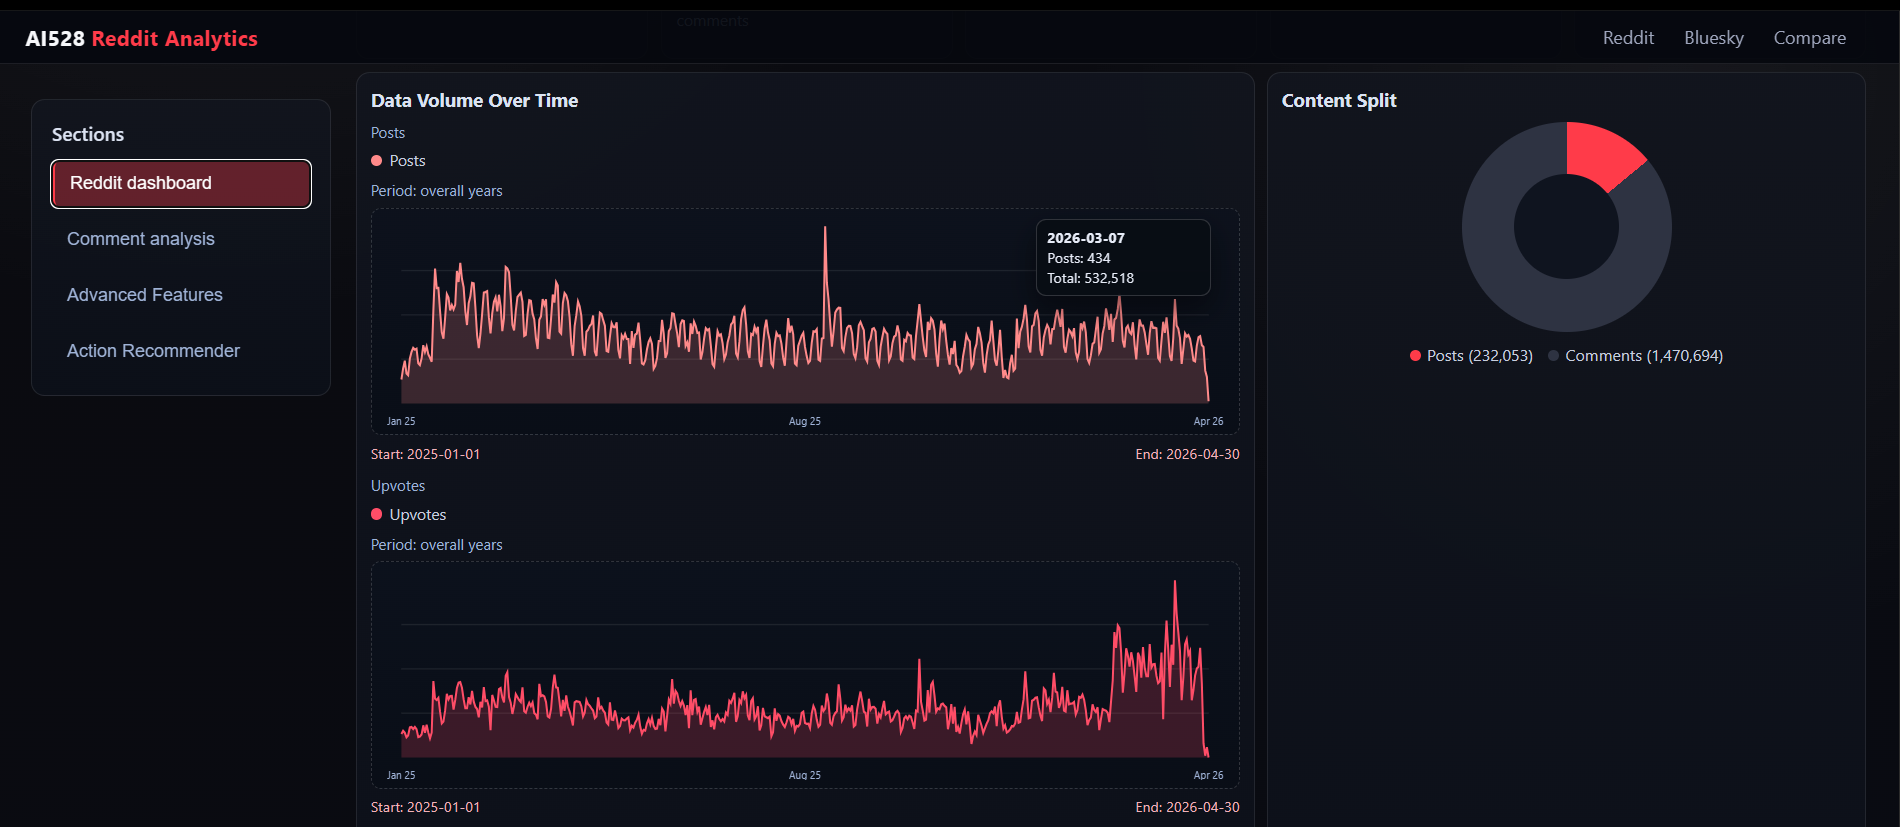
\includegraphics[width=\columnwidth]{reddit_overview.png}
  \caption{Reddit overview: volume trends and content split.}
\end{figure}

\section{Analytics Explanation}
\textbf{Reddit overview.} The main dashboard summarizes total posts, total engagement, average engagement per day, average score, and average comments. The time-series panels show posts, upvotes, and comments over time, while the donut chart separates posts and comments. The screenshot shows a comment-heavy dataset with 232,053 posts and 1,470,694 comments, indicating that discussion volume dominates original post volume.

\textbf{Comment analysis.} The comment page focuses on total comments, controversial comments, average comment upvotes, and average comment score. It also visualizes comment volume, controversial comment volume, non-controversial volume, weekly activity, and comment score split. In the screenshot, 36,956 comments are controversial, about 2.51\% of the 1.47M comments, so controversy is present but not dominant.

\textbf{Advanced features.} This section applies sentiment, word popularity, heatmaps, topic controversy, word sentiment versus engagement, and trend saturation. The heatmap groups top topics by month and lexicon sentiment. The keyword and controversy panels reveal which terms are both frequent and discussion-heavy. The trend saturation monitor detects topics whose activity peaked earlier and then declined, using per-word time series and slope-based checks.

\textbf{Action recommender.} The recommender accepts a proposed post title, evaluates lexicon sentiment, and applies deterministic decision rules. It also lists best topics to post about and topics to avoid. Best topics combine positive sentiment, normalized engagement, and positive rate; avoid topics combine negative sentiment strength, negative rate, and controversy. This directly supports the project goal: suggesting Reddit content that is likely to receive engagement while avoiding topics with high controversy or negative sentiment.

\begin{figure}[h]
  \centering
  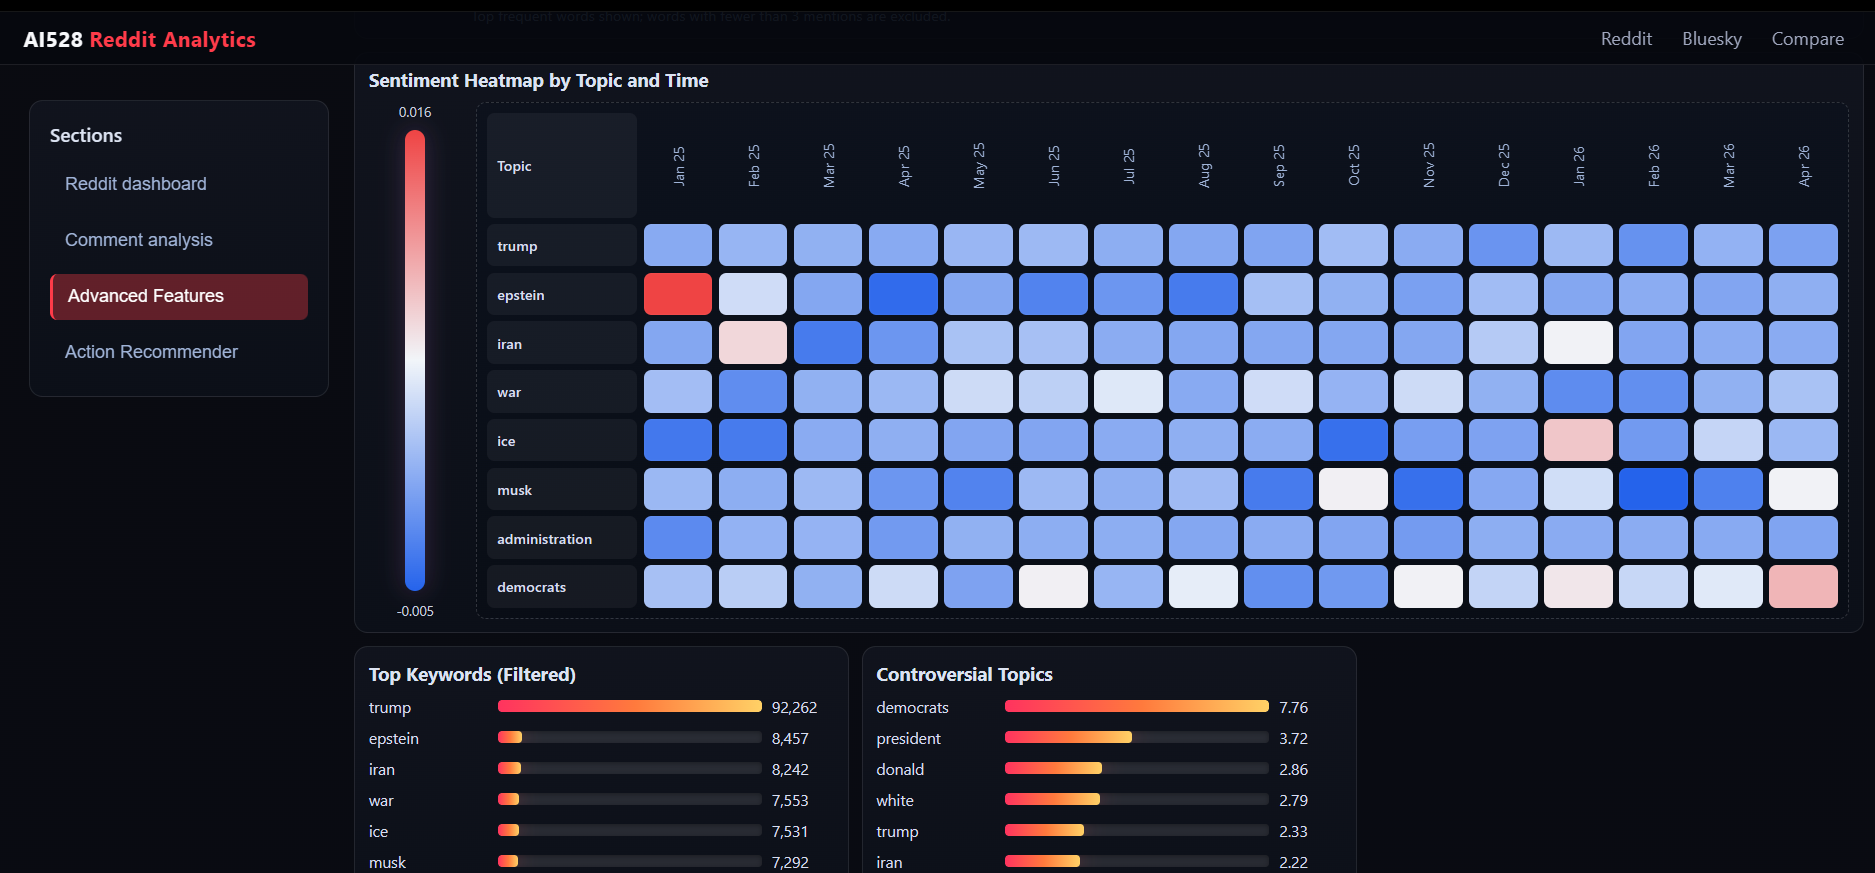
\includegraphics[width=\columnwidth]{advanced_heatmap.png}
  \caption{Advanced view: topic sentiment heatmap with keyword and controversy panels.}
\end{figure}

\section{Key Findings}
\begin{itemize}
  \item The dataset is highly discussion-oriented: comments outnumber posts by more than six times, so comment analytics are essential for understanding user reaction.
  \item Engagement is bursty. The post and upvote charts show clear spikes, especially around late August 2025 and early 2026, suggesting event-driven traffic rather than steady growth.
  \item Comment controversy is measurable but limited. The comment dashboard reports roughly 2.5\% controversial comments, while non-controversial comments form the overwhelming majority.
  \item Frequent political and news terms dominate Reddit activity. The screenshots show high-frequency keywords such as \textit{trump}, \textit{epstein}, \textit{iran}, \textit{war}, \textit{musk}, and \textit{administration}.
  \item Topic controversy is concentrated in political entities and current-affairs terms. The controversy panel highlights \textit{democrats}, \textit{president}, \textit{donald}, \textit{white}, \textit{trump}, and \textit{iran}.
  \item Trend saturation identifies fading topics. The monitor shows examples such as \textit{musk}, \textit{elon}, and \textit{tariffs} with early spikes followed by lower sustained activity.
  \item The dashboard is designed for explainability: each recommendation is backed by sentiment, engagement, negative rate, controversy, or trend behavior rather than only a final score.
\end{itemize}

\begin{figure}[h]
  \centering
  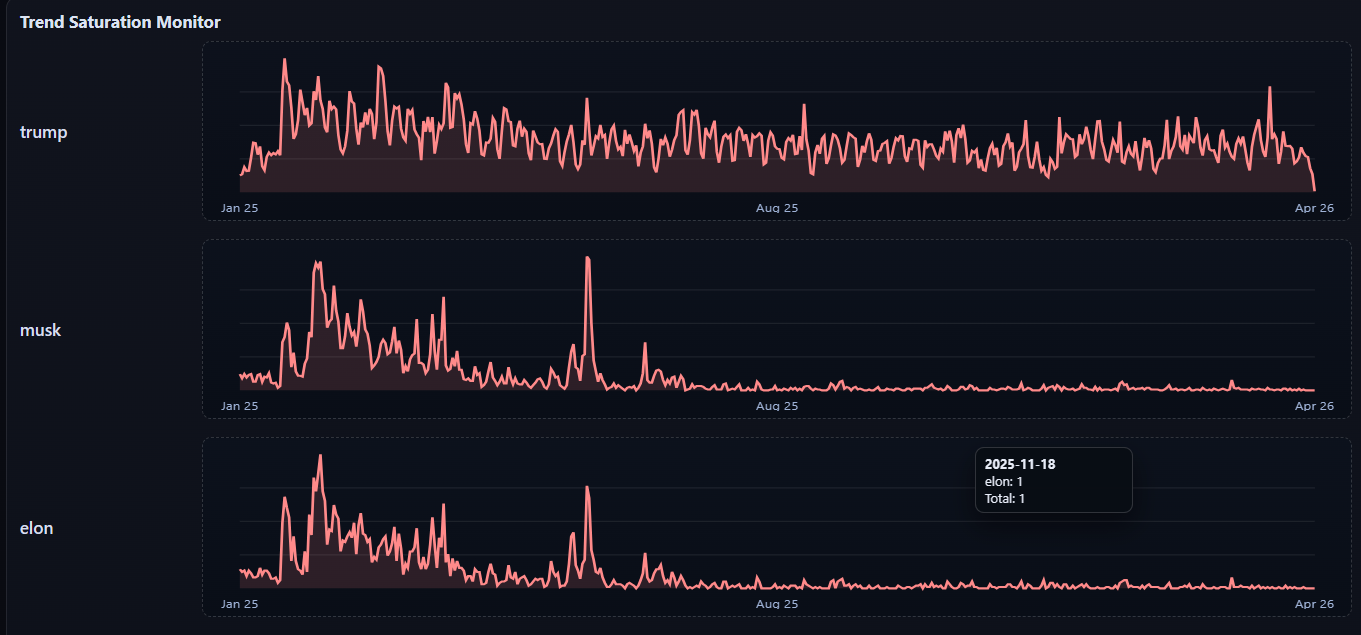
\includegraphics[width=\columnwidth]{trend_saturation.png}
  \caption{Trend saturation monitor showing fading topic activity.}
\end{figure}

\vspace{-0.2cm}
\section{Conclusion}
The dashboard provides an end-to-end Big Data analytics workflow: ingestion into SQLite through Spark-compatible scripts, API-level aggregation in FastAPI, lexicon-based sentiment analysis, vector retrieval support with Qdrant, and interactive React visualizations. The main analytical value is the combination of popularity, engagement, sentiment, controversy, and trend saturation into a single interface that supports actionable Reddit posting recommendations.

\end{document}
